% ----------------------------------------------------------
\chapter{Paleta de cores UnB}\label{anx:coresunb}
% ----------------------------------------------------------

A \cpageref{marcaunb.1} foi extraída do \emph{manual de identidade visual}\footnote{Disponível em \url{http://marca.unb.br}} da UnB.

\cleardoublepage

\newcounter{includepdfpage} % para referenciar no texto páginas pdf incluídas
\makepagestyle{simple}
\makeevenhead{simple}{\footnotesize\thepage}{}{}
\makeoddhead{simple}{}{}{\footnotesize\thepage}

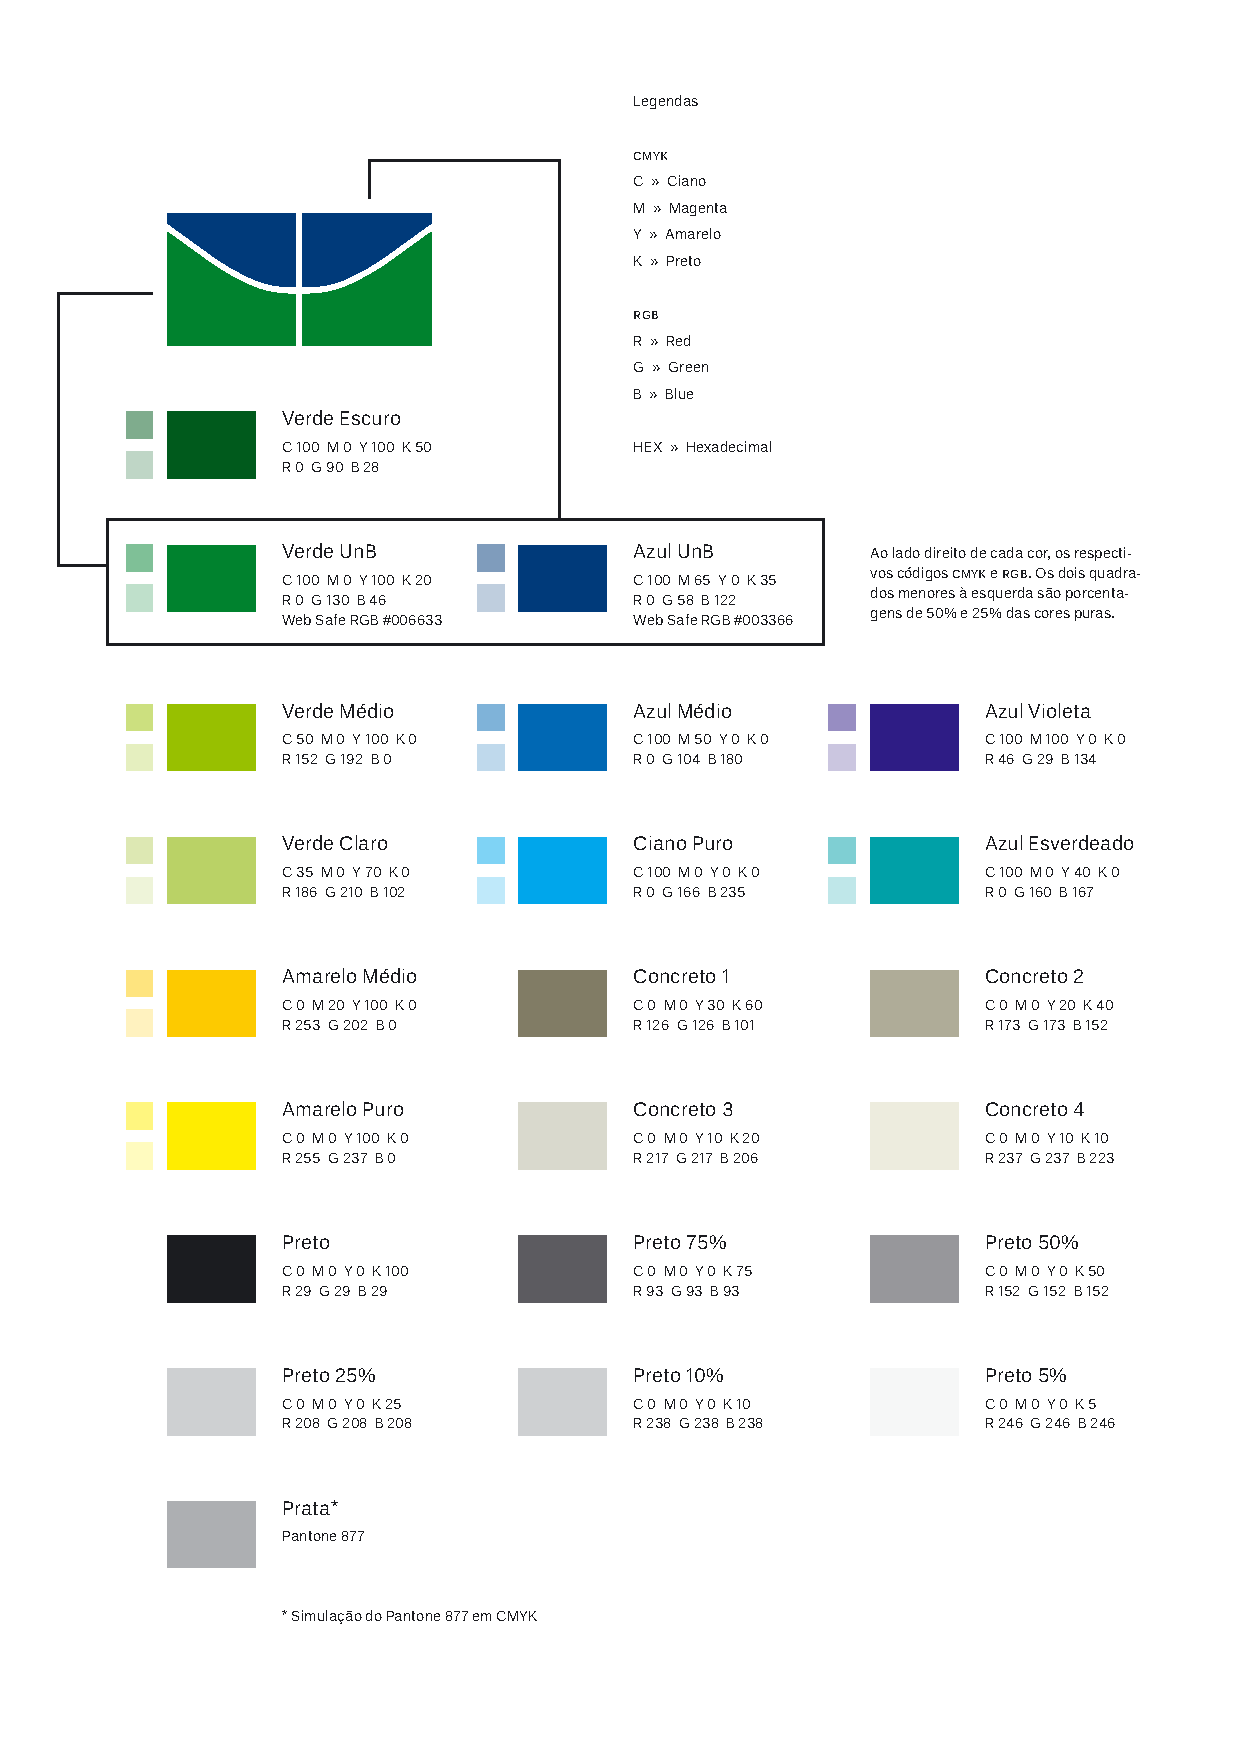
\includepdf[
    pages=-, % intervalo das páginas do arquivo pdf que serão incluídas
    scale=1, % controla o tamanho da página inserida
    pagecommand={\thispagestyle{simple} % imprime o número da página
    \refstepcounter{includepdfpage} % conta a página incluída
    \label{marcaunb.\theincludepdfpage} % marcaunb.n, n número da página
    },
    ]{unbtex-example/figuras/coresunb}

\cleardoublepage